\documentclass[a4paper, 12pt]{article}

\def \srcdir{tex/}
\def \picdir{pic/}
\def \tbldir{tex/tables/}

\input{\srcdir properties}
\input{\srcdir macros}

\title{
  Лабораторная работа \textnumero \input{\srcdir index}\\
  \textbf{\textquote{\input{\srcdir name}\unskip}}
}
\author{\input{\srcdir author}}
\date{\input{\srcdir date}}

\begin{document}

\maketitle\thispagestyle{fancy}

\subsection*{Цель работы}
Определить изменения температуры углекислого гааз при протекании через\
малопроницаемую перегородку при разных начальных значениях дваления и температуры,\
вычислить по результатам опытов коэффициентов Ван-Дер-Ваальса \textquote{$a$} и \textquote{$b$}. 

\subsection*{Оборудование}
\begin{itemize}[noitemsep]
  \item Трубка с пористой перегородкой
  \item Труба Дьюара
  \item Термостат
  \item Термометр
  \item Дифференциальная термопара
  \item Микровольтметр
  \item Балластный баллон
  \item Манометр
\end{itemize}

\section{Теоретическая часть}
Эффектом Джоуля–Томсона называется изменение температуры газа, медленно протекающего\
из области высокого в область низкого давления в условиях хорошей тепловой изоляции.\
В разреженных газах, которые приближаются по своим свойствам к идеальному газу, при\
таком течении температура газа не меняется. Эффект Джоуля–Томсона демонстрирует отличие\
исследуемого газа от идеального.

В работе исследуется изменение температуры углекислого газа при медленном его течении\
по трубке с пористой перегородкой. Трубка 1 хорошо теплоизолирована. Газ из области\
повышенного давления $ P_1 $ проходит через множество узких и длинных каналов пористой\
перегородки 2 в область с атмосферным давлением $ P_2 $. Перепад давления $ \Delta P = P_1 - P_2 $\
из-за большого сопротивления каналов может быть заметным даже при малой скорости\
течения газа в трубке. Величина эффекта Джоуля–Томсона определяется по разности температуры\
газа до и после перегородки.

Рассмотрим стационарный поток газа между произвольными сечениями \Rnum{1} и \Rnum{2}\
трубки (до перегородки и после нее). Пусть, для определенности, через трубку прошел
1 моль углекислого газа; $ \mu $ -- его молярная масса. Молярные объемы газа, его давления
и отнесенные к молю внутренние энергии газа в сечениях \Rnum{1} и \Rnum{2} обозначим\
соответственно $ V_1, P_1, U_1 $ и $ V_2, P_2, U_2 $. Для того чтобы ввести в трубку\
объем $ V_1 $, над газом нужно совершить работу $ A_1 = P_1V_1 $. Проходя через сечение \Rnum{2},\
газ сам совершает работу $ A_2 = P_2V_2 $. Так как через боковые стенки не происходит\
ни обмена теплом, ни передачи механической энергии, то
\label{1}\feq[]{A_1-A_2=\left(U_2+\frac{\mu v_2^2}{2}\right) - \left(U_1 + \frac{\mu v_1^2}{2}\right).}
В уравнении \eqref{1} учтено изменение как внутренней (первые члены в скобках), так\
и кинетической (вторые члены в скобках) энергии газа. Подставляя в \eqref{1} написанные\
выражения для $ A_1 $ и $ A_2 $ и перегруппировывая члены, найдем
\label{2}\feq[]{H_1-H_2=\left(U_1+P_1V_1\right) - \left(U_2 + P_2V_2\right) = \frac{1}{2} \mu \left(v^2_2-v^2_1\right).}

Сделаем несколько замечаний. Прежде всего отметим, что в процессе Джоуля–Томсона газ испытывает в пористой перегородке существенное трение, приводящее к ее нагреву. Потери энергии на нагрев трубки в начале процесса могут быть очень существенными и сильно искажают ход явления. После того как температура трубки установится и газ станет уносить с собой все выделенное им в пробке тепло, формула \eqref{1} становится точной, если, конечно, теплоизоляция трубки достаточно хороша и не происходит утечек тепла наружу через ее стенки.

Второе замечание связано с правой частью уравнения \eqref{2}. Процесс Джоуля–Томсона в чистом виде осуществляется лишь в том случае, если правой частью можно пренебречь, т. е. если макроскопическая скорость газа с обеих сторон трубки достаточно мала. У нас сейчас нет критерия, который позволил бы установить, когда это можно сделать. В силу сохранения энтропии в случае реального газа получаем:

\begin{equation}\label{3}
\mu_{д-т} = \frac{\Delta T}{\Delta P} \approx \frac{(2a/RT) - b}{C_P}.
\end{equation}

Из формулы \eqref{3} видно, что эффект Джоуля–Томсона для не очень плотного газа зависит от соотношения величин $ a $ и $ b $, которые оказывают противоположное влияние на знак эффекта. Если силы взаимодействия между молекулами велики, так что превалирует <<поправка на давление>>, то основную роль играет член, содержащий $ a $, и 

\[ \frac{\Delta T}{\Delta P} > 0, \]
т. е. газ при расширении охлаждается ($ \Delta T < 0 $, так как всегда $ \Delta P < 0 $). В обратном случае (малые $ a $)

\[ \frac{\Delta T}{\Delta P} < 0, \]
т. е. газ нагревается ($ \Delta T > 0 $, так как по-прежнему $ \Delta P < 0 $).

Этот результат нетрудно понять из энергетических соображений. Как мы уже знаем, у идеального газа эффект Джоуля–Томсона отсутствует. Идеальный газ отличается от реального тем, что в нем можно пренебречь потенциальной энергией взаимодействия молекул. Наличие этой энергии приводит к охлаждению или нагреванию реальных газов при расширении. При больших a велика энергия притяжения молекул. Это означает, что потенциальная энергия молекул при их сближении уменьшается, а при удалении -- при расширении газа -- возрастает. Возрастание потенциальной энергии молекул происходит за счет их кинетической энергии -- температура газа при расширении падает. Аналогичные рассуждения позволяют понять, почему расширяющийся газ нагревается при больших значениях $ b $.

Как следует из формулы \eqref{3}, при температуре \[ T_{\text{инв}} = \frac{2a}{Rb} \] коэффициент $ \mu_\text{Д--Т} $ обращается в нуль. По формулам связи параметров газа Ван-дер-Ваальса с критическими параметрами получаем: 

\begin{equation}\label{4}
T_\text{инв} = \frac{27}{4} T_\text{кр}.
\end{equation}

При температуре $ T_\text{инв} $ эффект Джоуля–Томсона меняет знак: ниже температуры инверсии эффект положителен ($ \mu_\text{Д--Т} > 0 $, газ охлаждается), выше $ T_\text{инв} $ эффект отрицателен ($ \mu_\text{Д--Т} < 0 $, газ нагревается).

\section{Ход работы}
Результаты измерений и расчета $\Delta T$ приведены в \textbf{таб. 1}.\ 
Формулы для расчета погрешности $\Delta T$:
\feq[]{\sigma_{\Delta T} = \Delta T \sqrt{\left(\frac{\sigma_U}{U}\right)^2 +  \left(\frac{\sigma_\xi}{\xi}\right)^2}}
Графики $\Delta T(\Delta P)$ приведены на \textbf{рис. 1---3}. Результаты расчета величин для\
построения графика $\mu_{д-т}(1/T)$ приведены в \textbf{таб. 2}, сам график --- на \textbf{рис. 4}.
Итоговые значения коэффициентов Ван-Дер-Ваальса:
\feq{a = (0.321 \pm 0.010)\ Н \cdot м^4/моль^2,\quad b = (154 \pm 8)\ см^3/моль.}
Температура инверсии:
\feq{T_i = \frac{2a}{Rb} = (500 \pm 30)\ К}

\stbl{final}{Значения величин для графика $\mu_{д-т}(T^{-1})$}

\stbl{main}{Основные измерения}
\svg[1]{20deg}{График зависимости $\Delta T(\Delta P)$ при $T = 20 ^\circ C$}
\svg[1]{30deg}{График зависимости $\Delta T(\Delta P)$ при $T = 30 ^\circ C$}
\svg[1]{50deg}{График зависимости $\Delta T(\Delta P)$ при $T = 50 ^\circ C$}
\svg[1]{final.svg}{График зависимости $\mu_{д-т}(T^{-1})$}

\begin{figure}[h]
  \begin{center}
    \fontsize{7}{8}\selectfont
    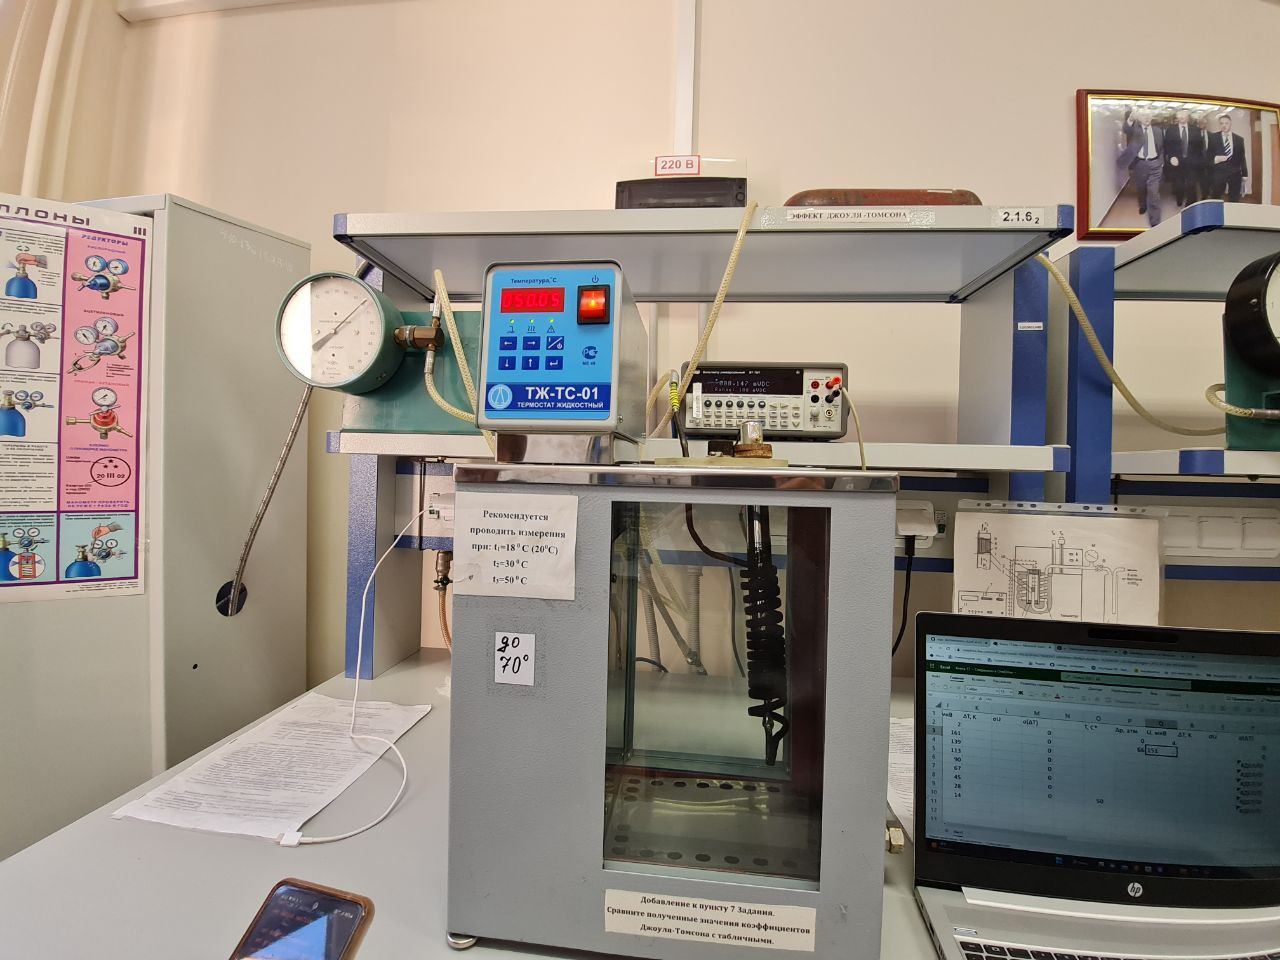
\includegraphics[scale=0.4]{include/equip.jpg}
    \caption{Установка}
  \end{center}
  \end{figure}

\subsection*{{Вывод}}
Коэффициент $a$ отличен от табличного примерно на $10\%$, коэффициент $b$
примерно в 4 раза больше.
\end{document}